\documentclass[12pt,a4paper]{report}
\usepackage[utf8]{inputenc}
\usepackage{amsmath}
\usepackage{amsfonts}
\usepackage{polski}
\usepackage{amssymb}
\usepackage{makeidx}
\usepackage{graphicx}
\setlength{\headheight}{0pt}
\setlength{\textheight}{23.5cm}
\setlength{\textwidth}{15.92cm}
\setlength{\footnotesep}{5mm}
\setlength{\footskip}{10mm}
\setlength{\oddsidemargin}{0mm}
\setlength{\evensidemargin}{0mm}
\setlength{\topmargin}{0mm}
\setlength{\headsep}{5mm}
\setlength{\parindent}{0mm}
\setlength{\parskip}{2.5mm}
\author{Maciej Skarbek \\Nr albumu: 271088}
\title{{\Huge \textbf{Specyfikacja implementacyjna \\,,gentex"}}}

\begin{document}
\maketitle

\section*{Wprowadzenie} Celem projektu jest stworzenie aplikacji w języku C, która będzie generować teksty wyjściowe na podstawie analizy innych tekstów wykorzystując przy tym łańcuchy Markova. Przy tworzeniu programu korzystać będziemy z systemu kontroli wersji git.

\section*{Opis modułów}

	\subsection*{managment} Rozpoznaje argumenty wywołań i steruje innymi modułami. Zawiera funkcje "main".
	
	\subsection*{store} Przechowuje macierz przejść z podziałem na prefiksy i sufiksy. Implementacja drzewa.
	
	\subsection*{generation} Generuje tekst wynikowy i zapisuje go do pliku.
	
	\subsection*{reading} Odczytuje teksty podane przez użytkownika. Analizuje je dzieląc na prefiksy i sufiksy a następnie przekazuje do modułu "store".
	
	\subsection*{backup} Tworzy i umożliwia wczytanie plików pośrednich z których w przyszłości można generować teksty wynikowe.
	
	\subsection*{stats} Tworzy statystyki łączone dla tekstów bazowych i oddzielną statystykę dla tekstu wynikowego (prawdopodobieństwo wystąpienia pojedyńczego słowa, n-gramu z jakich został wygenerowany tekst i wskaźnik PMI).
	
	\subsection*{error} Obsługuje błędy zaistniałe podczas działania.
	
\section*{Opis najważniejszych funkcji i struktur} 

	\subsection*{managment}
	
		\begin{itemize}
			
			\item void add(char **prefix, char * suffix) \\
			Rozpoznanie argumentów wywołania i przekazanie sterowania do odpowiednich modułów.
			
		\end{itemize}
	
	\subsection*{store} 
	
		\begin{itemize}
			\item Struktury \\
			$\begin{array}{lll}
				typedef struct \{ 				& typedef struct node \{ 					& typedef struct \{ \\ 
				\hspace{1em}char ** prefix; 	& 	\hspace{1em}ngram * g; 					& \hspace{1em}	tree\_t t; \\ 
				\hspace{1em}char ** suffix; 	& 	\hspace{1em}struct node *left, *right; 	& \hspace{1em}	int number\_gram; \\ 
					\hspace{1em}int size\_s; 	& \} node\_t, *tree\_t; 					& 	\hspace{1em}int size; \\ 
						\hspace{1em}int n\_s; 	&  											& \hspace{1em}	ngram** tab; \\ 
					\} ngram; 					&  											& 	\hspace{1em}int n\_s\_max; \\ 
												&  											& \} store;
			\end{array} $ \linebreak
			
			Tworzone jest drzewo do przechowywania prefiksów i sufiksów jak również tablica w której będą wskaźniki do komurek drzewa. Tablica będzie używana przy losowaniu prefiksów jak również przy tworzeniu pliku pośredniego (gdybyśmy chcieli stworzyć plik pośredni z drzewa był by on posortowany i przy wczytywaniu zamiast drzewo powstała by nam lista co znacząco wydłużyło by czas pracy programu).
			
			\item tree\_t insert( tree\_t t, char **prefix, char * suffix )\\
			Wstawia do drzewa prefiksy i sufiksy, jeśli prefiks juz istnieje to dopisuje tylko sufiks. Dodaje również wzkaźnik na "ngram" do "tab".
			
			\item void add\_from\_backup(char **prefix, char **suffix, int n\_s) \\
			Dodaje prefiks i całą listę sufiksów do drzewa.
			
			\item ngram* rand\_prefix() \\
			Losuje prefiks.
			
			\item char* rand\_suffix(char** prefix)\\
			Losuje sufiks dla podanego prefiksu.
			
		\end{itemize}
	
	\subsection*{generation} 
		\begin{itemize}
			
			\item void generation()\\
			Generuje tekst wynikowy i zapisuje go do pliku.
			
		\end{itemize}
	
	\subsection*{reading} 
		\begin{itemize}
			
			\item void reading( char * name\_file)\\
			Czyta podany plik, dzieli na prefiksy i sufiksy a następnie przekazuje do "store" i "stat".
			
		\end{itemize}
	
	\subsection*{backup} 
		\begin{itemize}
			
			\item void backup()\\
			Tworzy plik wczytuje i tworzy plik pośredni.
			
		\end{itemize}
	\subsection*{stats}
		\begin{itemize}
			
			\item void stat\_add\_word(char * word) \\
			Dodaje pojedynczy wyraz do drzewa ze statystykami (zlicza ilośc wystąpień).
			
			\item void stat\_add\_ngram(char** prefix,char * suffix)\\
			Dodaje n-gram do drzewa ze statystykami i zlicza ilość wystąpień.
			
			\item double get\_probability(tree\_stat t, char * word)\\
			Liczy prawdopodobieństwo dla n-gramu.
			
			\item long double get\_pmi(char* wngram)\\
			Liczy wskaźnik PMI dla n-gramu.
			
			\item void write\_stat( char * name\_file\_stat)\\
			Zapisuje statystyki do podanego pliku.
			
		\end{itemize}
	\subsection*{error} 
		\begin{itemize}
			
			\item void fatal(int err, const char *msg)\\
			Dostaje wyrażenie logiczne "err" i w przypadku potwierdzenia wystąpienia błędu pokazuje wiadomość "msg" i np. zamyka program.
		\end{itemize}

\section*{Testowanie}

	\subsection*{Użyte narzędzia}
	
		\subsubsection*{time} Polecenie time do pomiaru czasu działania programu aby wybrać optymalny algorytm jaki zaimplementujemy.
		
		\subsubsection*{valgrind} Narzędzie do debugowania pamięci i wykrywania wycieków pamięci.

	\subsection*{Sposób testów} Testy będą wykonywane dla pojedynczych funkcjonalności programu, dla całych modułów a następnie po przyłączeniu kolejnego modułu zostaną wykonane kompleksowe testy całego programu. Szczególną uwagę należy zwrócić na punkty krytyczne w których możemy spodziewać sie błędów.

	\subsection*{Punkty krytyczne} 
		\begin{itemize}
			
			\item Bardzo duże pliki wejściowe
			\item Puste pliki wejściowe
			\item Bardzo małe pliki wejściowe (np 2 słowa)
			\item Błędnę wywołanie programu
			\item Podanie pliku do zapisu który już istnieje
			\item Mała ilość pamięci urządzenia na którym zostanie uruchomiony program
			\item Wycieki pamięci
			
		\end{itemize}

\section*{Diagram modułów} \begin{figure}
\centering
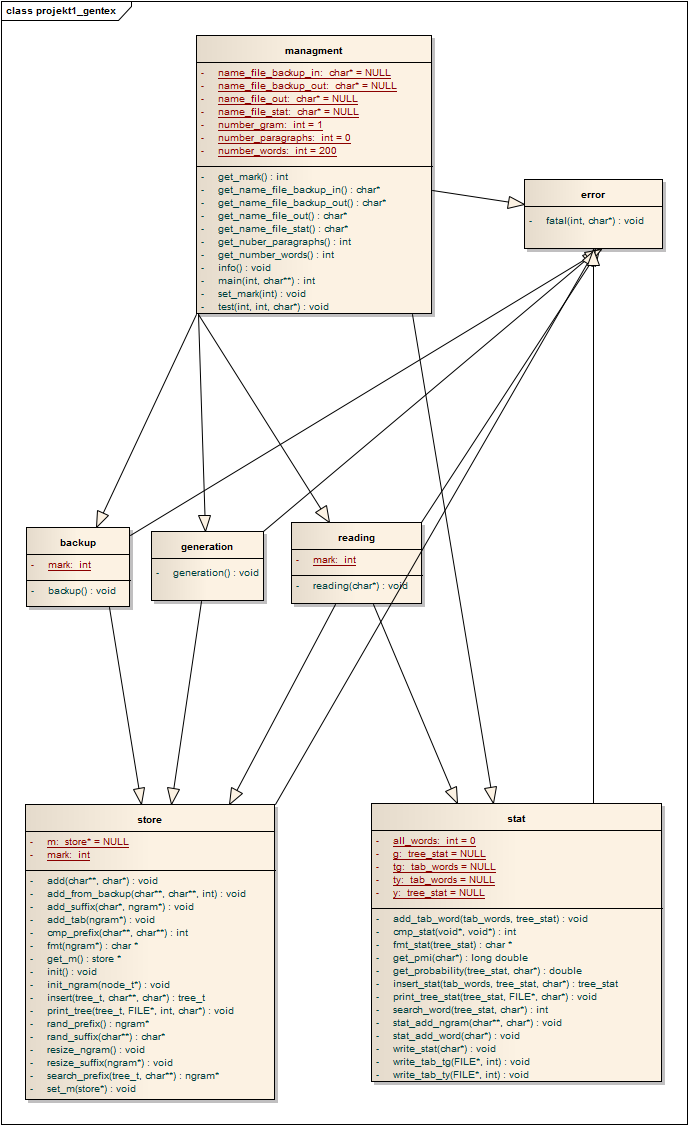
\includegraphics[width=0.89\linewidth]{E:/Copy/Studia/Git/projekt1_gentex/projekt1_gentex1}
\caption{}
\label{fig:projekt1_gentex1}
\end{figure}

\end{document}